\chapter{Referencial Teórico}
\label{cap:referencial_teorico}

Este capítulo estabelece o arcabouço teórico e conceitual necessário para a compreensão da modelagem preditiva aplicada à administração tributária. A discussão inicia-se com a definição da análise tributária baseada em dados (\textit{Tax Analytics}) e sua isomorfia com a pontuação de crédito (\textit{Credit Scoring}) bancária, destacando as especificidades do setor público. Em seguida, apresentam-se os fundamentos algorítmicos dos métodos de conjunto (\textit{ensemble}), do \textit{Gradient Boosting} e do XGBoost. Na sequência, analisa-se o dilema fundamental entre a capacidade de generalização de modelos de caixa-preta e a interpretabilidade intrínseca de modelos lineares, bem como as implicações econômicas dessa escolha estratégica, os riscos de viés, o desbalanceamento dos dados e as métricas usadas para avaliar a performance do modelo e detectar tratamento desigual entre grupos. Por fim, fundamenta-se a Inteligência Artificial Explicável como requisito de governança, detalhando as metodologias SHAP e LIME sob a ótica da consistência, segurança jurídica e funcionamento algorítmico.

\section{Da análise tributária baseada em dados à pontuação de crédito: isomorfia e especificidades no setor público}
\label{sec:tax_analytics}

A gestão da Dívida Ativa no setor público tem evoluído de um paradigma puramente cartorial e reativo para uma abordagem analítica e estocástica, denominada na literatura contemporânea como análise tributária baseada em dados (\textit{Tax Analytics}). Do ponto de vista da ciência de dados, o problema de classificar um contribuinte quanto à probabilidade de recuperação de seu débito é tecnicamente isomorfo ao problema de pontuação de crédito (\textit{Credit Scoring}) enfrentado por instituições financeiras \cite{changCreditRiskPrediction2024, noriegaMachineLearningCredit2023}. Em ambos os cenários, o objetivo central é mitigar a assimetria de informação estimando a probabilidade de inadimplência (\textit{default}) com base em padrões históricos de comportamento.

\citeonline{zouInterpretableCreditScoring2025} destacam que, no ecossistema financeiro moderno, a avaliação precisa de solvência depende da capacidade de capturar relações não-lineares e comportamentos ``caóticos'' entre as variáveis do devedor, superando as limitações dos modelos estatísticos clássicos. 

Contudo, há uma distinção teleológica fundamental: enquanto instituições privadas operam sob a lógica de minimização de risco financeiro privado, a administração tributária opera sob os princípios da impessoalidade e da eficiência arrecadatória.  O \textit{rating} da SEFAZ-DF não apenas classifica um risco, mas modula o poder de execução do Estado.  Nesse contexto, o uso de modelagem avançada e fontes de dados alternativas é crucial para aprimorar a acurácia da avaliação de risco, garantindo que a cobrança seja direcionada de forma eficiente e justa \cite{hlongwaneEnhancingCreditScoring2024}.

\begin{figure}[H]
    \centering
    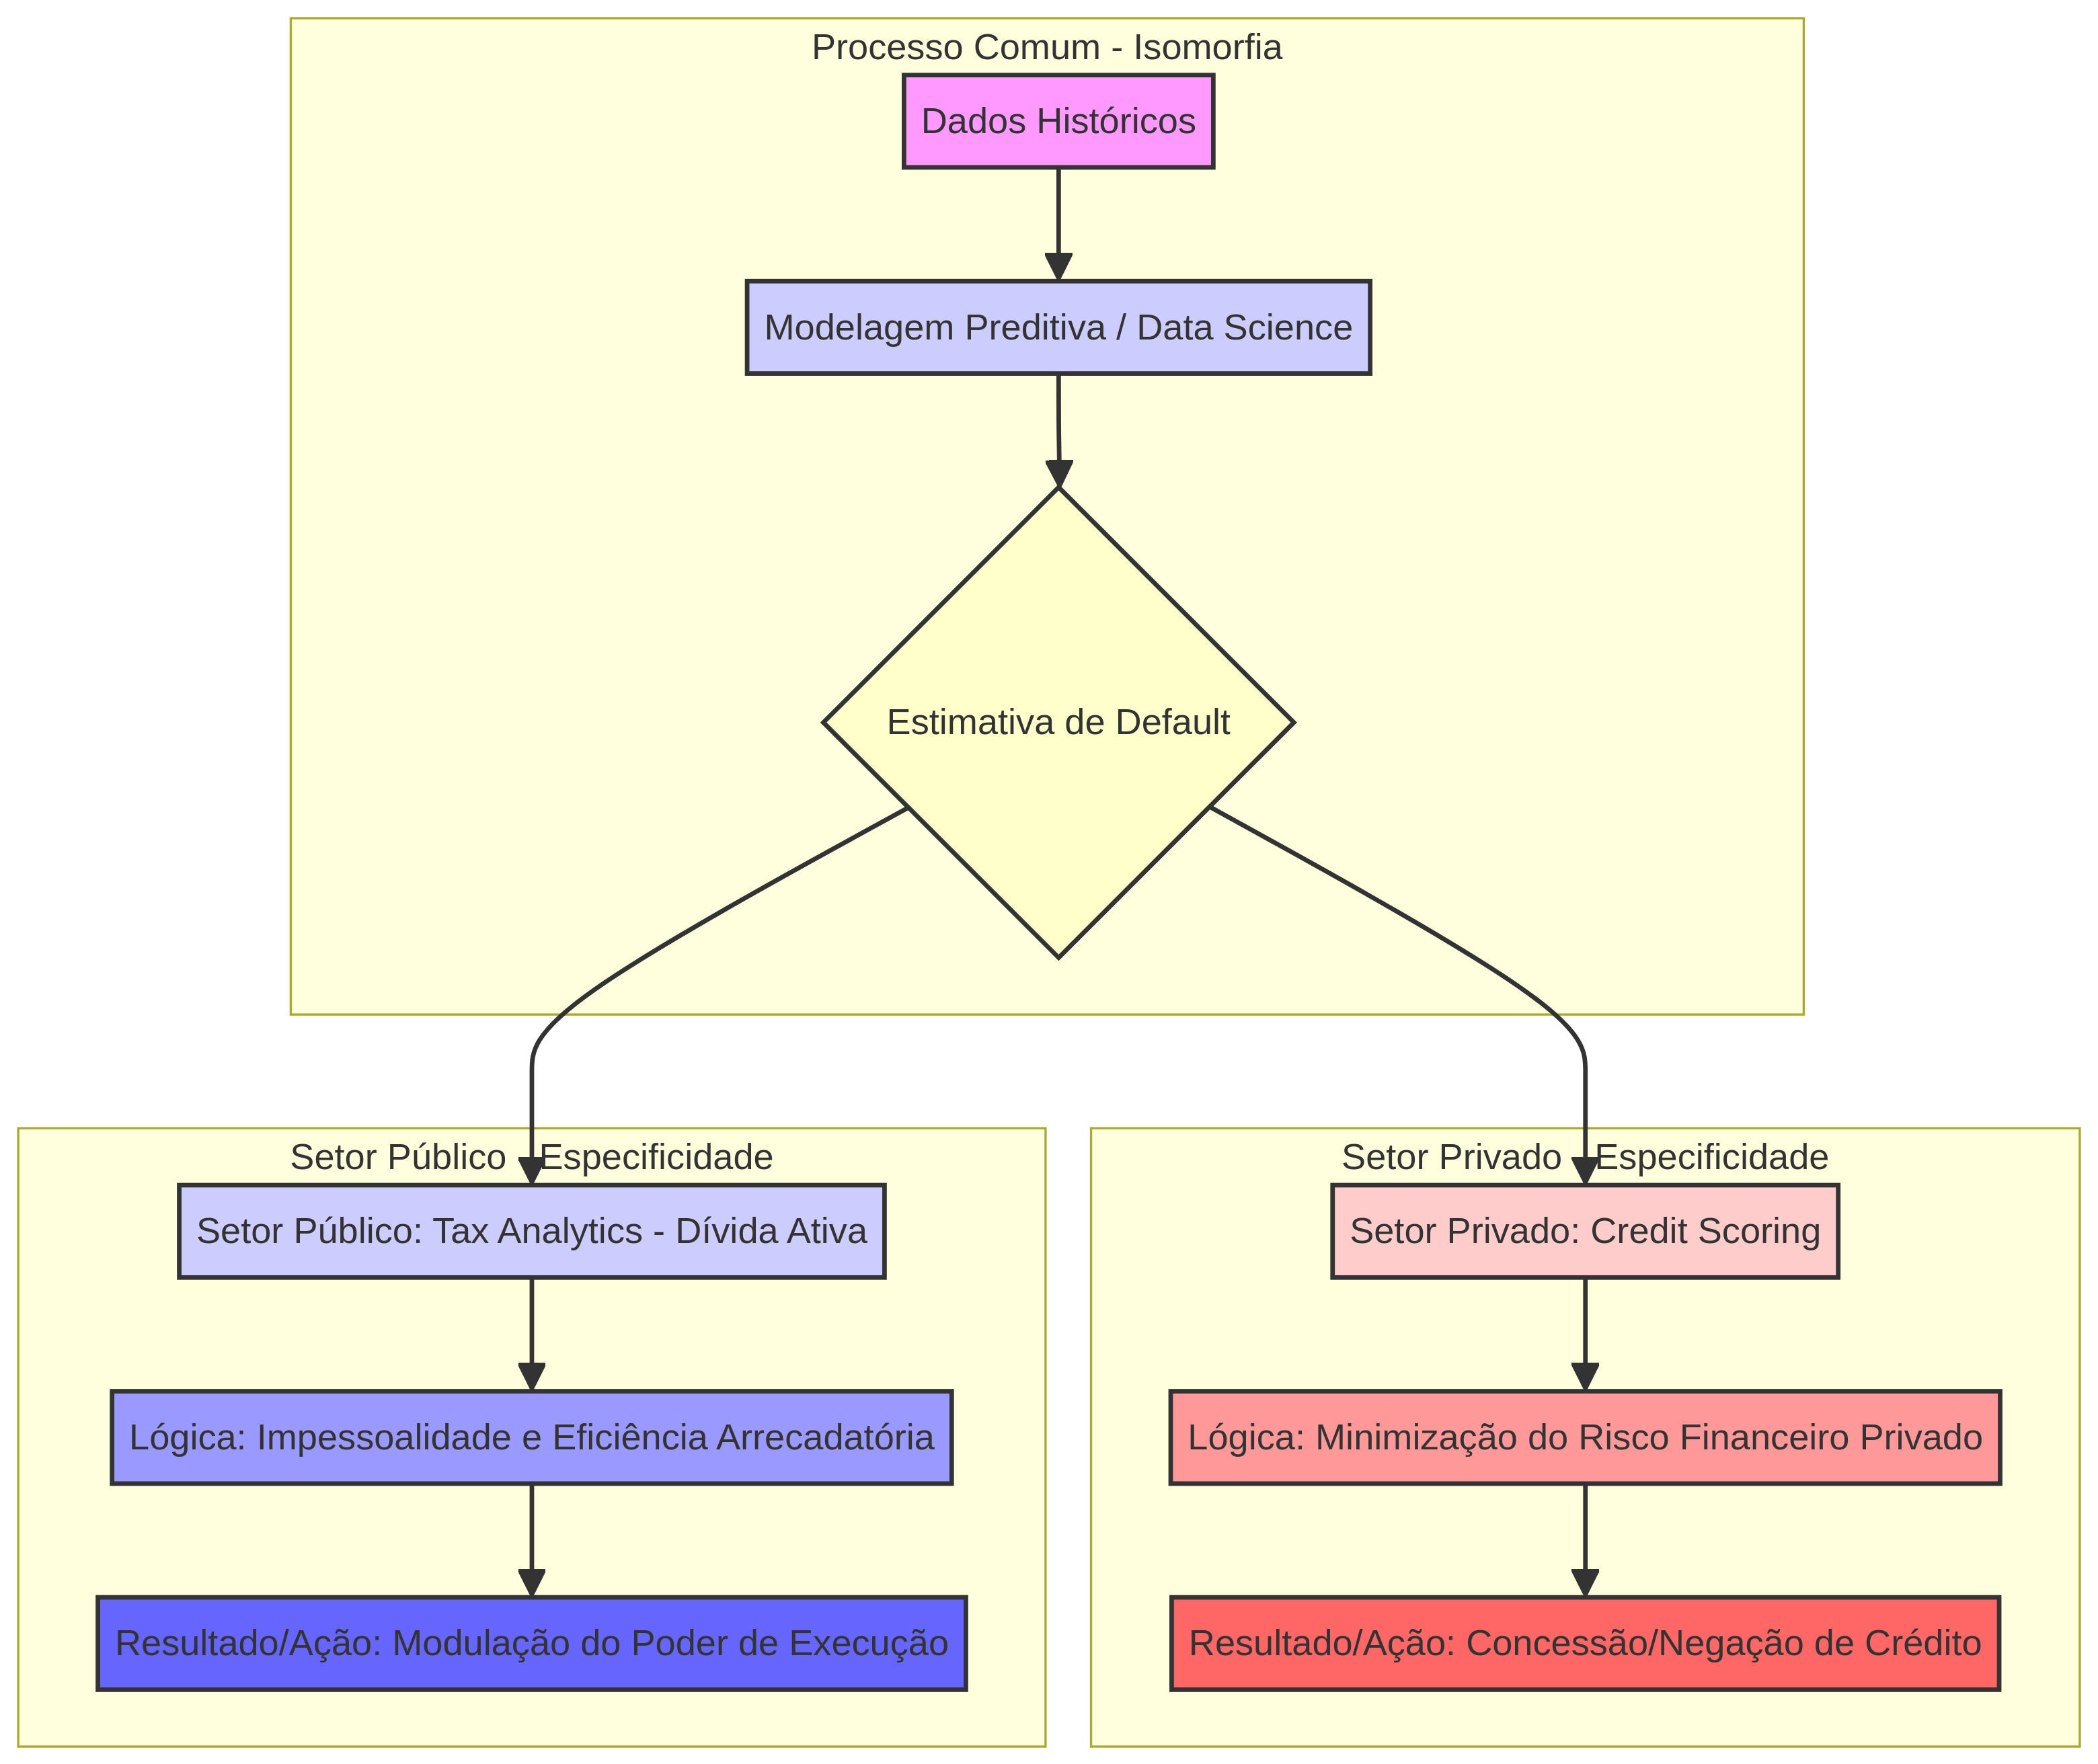
\includegraphics[width=0.85\textwidth]{figuras/tax_analytics_credit_scoring.png}
    \caption[Isomorfia entre análise tributária baseada em dados e pontuação de crédito]{Isomorfia e especificidades entre a análise tributária baseada em dados (setor público) e a pontuação de crédito (setor privado). O bloco superior mostra o processo comum aos dois contextos: dados históricos alimentam um modelo preditivo que estima a probabilidade de inadimplência. Os blocos inferiores mostram onde eles divergem: no setor público, a decisão segue os princípios da impessoalidade e da eficiência arrecadatória e serve para modular a atuação de cobrança do Estado; no setor privado, segue a lógica de minimização do risco financeiro e resulta na concessão ou negação de crédito.}
    \label{fig:flow_tax_analytics}

\end{figure}

\section{Fundamentos Algorítmicos: Métodos de Conjunto (\textit{Ensemble}) e \textit{Gradient Boosting}}
\label{sec:gbdt}

A escolha da SEFAZ-DF pelo uso de \textit{Gradient Boosting}, especificamente o algoritmo XGBoost, para a classificação da Dívida Ativa não é arbitrária. O \textit{Gradient Boosting} é uma técnica de aprendizado de máquina baseada na combinação sequencial de modelos simples, geralmente árvores de decisão, em que cada novo modelo busca corrigir os erros cometidos pelos anteriores. Na literatura de ciência de dados aplicada a dados tabulares (estruturados em linhas e colunas, típicos de bases fiscais), os métodos de conjunto (\textit{ensemble}) baseados em árvores de decisão apresentam performance de destaque em termos de acurácia preditiva \cite{schwartzEnhancingMLModels2025,friedman2001greedy}.

\subsection{A Lógica dos Métodos de Conjunto}
Os métodos de conjunto (\textit{ensemble}) partem da premissa de que a combinação de múltiplos modelos simples, denominados \textit{weak learners} ou aprendizes fracos, resulta em um modelo final mais robusto e preciso do que qualquer um dos componentes individuais. A teoria por trás dessa abordagem remete ao conceito de ``sabedoria das multidões'': erros individuais tendem a ser cancelados quando as predições são agregadas \cite{hastieElementsStatisticalLearning2009}.

Existem duas estratégias principais de métodos de conjunto:
\begin{enumerate}
    \item \textbf{Bagging (agregação por amostragem):} Os modelos são treinados de forma paralela e independente, e o resultado final é a média (regressão) ou o voto majoritário (classificação). O exemplo clássico é o \textit{Random Forest}. O objetivo principal do Bagging é reduzir a \textbf{variância} do modelo, evitando \textit{overfitting}.

    \item \textbf{Boosting (aprendizado sequencial):} Os modelos são treinados de forma \textbf{sequencial}. Cada novo modelo tenta corrigir os erros cometidos pelos modelos anteriores. O objetivo principal do Boosting é reduzir o \textbf{viés} do modelo, evitando \textit{underfitting}. É nesta categoria que se enquadra a metodologia da SEFAZ-DF.
\end{enumerate}

\begin{figure}[H]
  \centering
  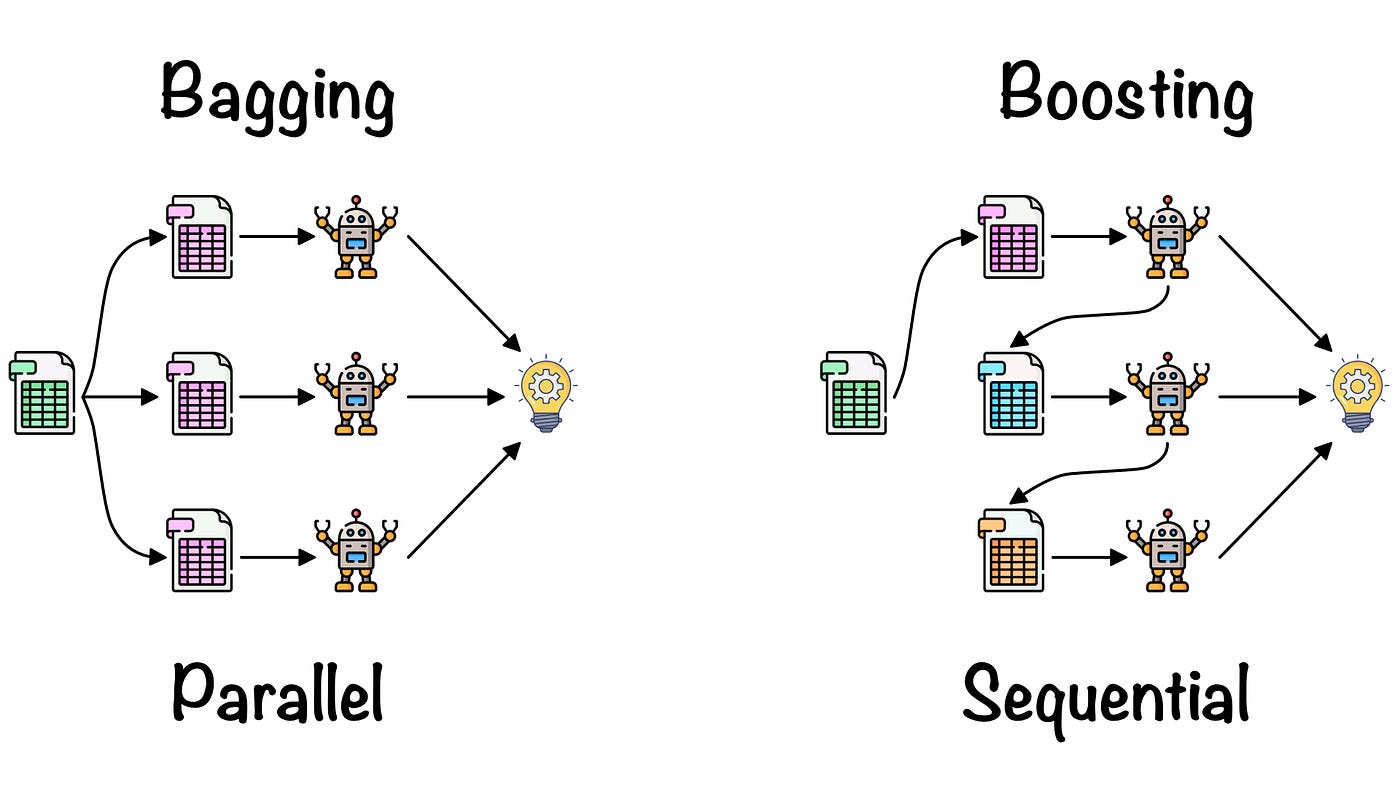
\includegraphics[width=0.9\textwidth]{figuras/baggingxboosting.jpg}
  \caption[Diferença estrutural entre \textit{Bagging} e \textit{Boosting}]{Diferença estrutural entre as duas estratégias de \textit{ensemble}. À esquerda, no \textit{Bagging}, a base original (tabela verde) é reamostrada em vários subconjuntos, e cada um treina um modelo de forma paralela e independente; as predições são combinadas por média ou voto (lâmpada). À direita, no \textit{Boosting}, os modelos são treinados em sequência: cada um recebe os dados reponderados conforme os erros do anterior (tabelas de cores diferentes) e as predições são somadas. O XGBoost, usado no Rating da SEFAZ-DF, pertence à segunda família.}
  \label{fig:ensemble_comparison}

  \small{Fonte: Elaborado pelos autores com base em \citeonline{hastieElementsStatisticalLearning2009}.}
\end{figure}

\subsection{\textit{Gradient Boosting Decision Trees}}
O \textit{Gradient Boosting}, formalizado por \citeonline{friedman2001greedy}, é uma técnica de otimização numérica no espaço de funções. O termo \textit{gradient}, em inglês, refere-se ao gradiente da função de perda, isto é, à direção de maior variação do erro do modelo. Ao contrário de modelos estatísticos tradicionais que buscam otimizar parâmetros, o \textit{Gradient Boosting} otimiza a própria função de predição $F(x)$.

O processo ocorre em iterações. Em cada etapa $m$, um novo modelo de árvore de decisão $h_m(x)$ é adicionado para minimizar a função de perda $L$ (do inglês \textit{loss function}), seguindo a direção do gradiente negativo dessa perda. Matematicamente, o modelo é atualizado da seguinte forma:

\begin{equation}
    F_{m}(x) = F_{m-1}(x) + \eta \cdot h_m(x)
\end{equation}

Onde:
\begin{itemize}
    \item $F_{m}(x)$ é o modelo atualizado na iteração $m$.
    \item $F_{m-1}(x)$ é o modelo da iteração anterior.
    \item $h_m(x)$ é a nova árvore treinada para prever os resíduos (erros) do modelo anterior.
    \item $\eta$ (eta) é a taxa de aprendizado (\textit{learning rate}), que controla a contribuição de cada árvore para evitar o ajuste excessivo aos dados de treino.
\end{itemize}

Para a gestão fiscal, isso significa que o modelo começa com uma predição rudimentar sobre a recuperação da dívida e, a cada nova árvore adicionada, refina sua compreensão sobre os casos mais difíceis, aumentando progressivamente a precisão da classificação nos Ratings A, B, C ou D.

\subsection{XGBoost: O Padrão da Indústria}
O documento metodológico da SEFAZ-DF cita explicitamente o uso do \textbf{XGBoost} (\textit{eXtreme Gradient Boosting}). Desenvolvido por \citeonline{chenXGBoostScalableTree2016}, o XGBoost é uma implementação otimizada do \textit{Gradient Boosting Decision Trees}, projetada para eficiência computacional e capacidade de representação de relações complexas.

Nesse contexto, o XGBoost diferencia-se do \textit{Gradient Boosting} tradicional por três inovações relevantes para o contexto tributário:

\begin{enumerate}
    \item \textbf{Regularização na Função Objetivo:} O XGBoost adiciona termos de regularização ($L1$ e $L2$) diretamente na função que está sendo otimizada. Isso penaliza árvores muito complexas, prevenindo que o modelo ``decore'' as dívidas específicas do passado e falhe em generalizar para novas dívidas (o problema do \textit{overfitting}).

    \item \textbf{Tratamento de Esparsidade (\textit{Sparsity-Aware}):} Dados fiscais frequentemente possuem valores ausentes. O XGBoost aprende automaticamente a melhor direção (esquerda ou direita na árvore) para seguir quando encontra um dado faltante, sem a necessidade de imputação artificial prévia.

    \item \textbf{Processamento Paralelo:} Embora o Boosting seja sequencial, o XGBoost paraleliza a construção de cada árvore, permitindo treinar modelos em milhões de registros de dívida ativa com rapidez.
\end{enumerate}

\subsection{LightGBM: Eficiência e Escalabilidade}
Embora a SEFAZ-DF utilize prioritariamente o XGBoost, a literatura recente aponta o \textbf{LightGBM} (\textit{Light Gradient Boosting Machine}), desenvolvido pela Microsoft, como uma alternativa eficiente, frequentemente utilizada em conjunto para validação cruzada \cite{ke2017lightgbm}.

A principal diferença do LightGBM é a estratégia de crescimento da árvore. Enquanto o XGBoost cresce a árvore por níveis (\textit{level-wise}), o LightGBM cresce por folhas (\textit{leaf-wise}), expandindo apenas o ramo que resulta na maior redução da perda. Isso torna o LightGBM mais rápido e capaz de lidar com volumes massivos de dados, embora exija maior cuidado com a configuração de hiperparâmetros para evitar sobreajuste em conjuntos de dados menores \cite{changCreditRiskPrediction2024}. Embora o LightGBM seja apresentado como referência técnica relevante, sua implementação experimental não faz parte do escopo deste trabalho, que se concentra na validação do modelo baseado em XGBoost e na aplicação de técnicas de explicabilidade.


\section{O Dilema Variância-Viés e a Opacidade Algorítmica na Administração Tributária}
\label{sec:tradeoff}

A adoção de Inteligência Artificial na gestão fiscal impõe um dilema fundamental conhecido na estatística como dilema viés-variância (\textit{bias-variance trade-off}). Na prática administrativa, isso se traduz em uma tensão entre a acurácia, entendida como a capacidade de acertar a previsão de recuperação do crédito, e a interpretabilidade, entendida como a capacidade de explicar o motivo da previsão \cite{rudinStopExplainingBlack2019}.

\subsection{A Natureza do Dilema entre Acurácia e Interpretabilidade}

Como modelo de referência para compreender a escolha pelo \textit{Gradient Boosting}, é essencial analisar o funcionamento da Regressão Logística, tradicionalmente utilizada em contextos de pontuação de crédito (\textit{Credit Scoring}).

A Regressão Logística é um modelo paramétrico que estima a probabilidade de um evento binário, como a inadimplência, mapeando as variáveis de entrada para uma função sigmoide. A função sigmoide é uma função matemática que transforma qualquer valor real em um número entre 0 e 1, permitindo interpretar a saída do modelo como probabilidade. Diferentemente da regressão linear, que prevê valores contínuos, a Regressão Logística transforma a soma ponderada das variáveis explicativas em um valor entre 0 e 1, conforme ilustrado na Figura \ref{fig:fluxograma_lr} \cite{hastieElementsStatisticalLearning2009}.

\begin{figure}[H]
    \centering
    % Substitua 'nome_da_sua_imagem.png' pelo arquivo que você enviou
    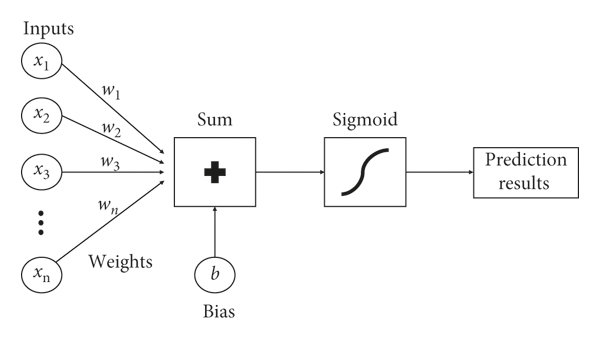
\includegraphics[width=0.9\textwidth]{figuras/Flowchart-of-logistic-regression.png} 
    \caption[Fluxo de processamento da Regressão Logística]{Fluxo de processamento da Regressão Logística. Cada variável de entrada $x_1, \dots, x_n$ é multiplicada por um peso $w_1, \dots, w_n$; os produtos são somados ao intercepto $b$ (\textit{bias}), e o resultado passa pela função sigmoide, que o converte em uma probabilidade entre 0 e 1. Como cada peso indica diretamente quanto a variável aumenta ou reduz a probabilidade, o modelo é considerado interpretável por construção (caixa-branca).}
    \label{fig:fluxograma_lr}
\end{figure}

Matematicamente, o modelo assume que existe uma relação linear entre as variáveis independentes e o logaritmo das chances (\textit{log-odds}) do evento. Essa característica o torna um modelo de caixa-branca: ao analisar os coeficientes $\beta$, isto é, os pesos atribuídos pelo modelo a cada variável explicativa, o auditor sabe exatamente o quanto cada variável aumentou ou diminuiu a probabilidade final \cite{hastieElementsStatisticalLearning2009}.

\noindent\textbf{Análise comparativa: por que não usar Regressão Logística?}

Apesar de sua transparência intrínseca, a Regressão Logística apresenta limitações severas para o problema da Dívida Ativa. A Tabela \ref{tab:vantagens_lr} resume as características do método.

\begin{table}[H]
\centering
\caption[Vantagens e desvantagens da Regressão Logística]{Vantagens (coluna da esquerda) e desvantagens (coluna da direita) da Regressão Logística quando aplicada à classificação de créditos tributários. Cada linha opõe um ponto forte a uma limitação relacionada: a interpretabilidade direta tem como contrapartida a suposição de relações lineares, o que explica por que a SEFAZ-DF optou por um modelo não linear.}
\label{tab:vantagens_lr}
\begin{tabular}{|p{0.45\linewidth}|p{0.45\linewidth}|}
\hline
\textbf{Vantagens} & \textbf{Desvantagens} \\
\hline
\textbf{Interpretabilidade Direta:} Os pesos (coeficientes) indicam a direção e magnitude do impacto de cada variável. & \textbf{Linearidade Restritiva:} Assume que as relações são lineares. Falha em capturar padrões complexos (ex: a dívida só é risco se associada a um setor específico). \\
\hline
\textbf{Baixo Custo Computacional:} Treinamento rápido e eficiente. & \textbf{Alto Viés (\textit{Underfitting}):} Tende a simplificar excessivamente a realidade fiscal, ignorando nuances do comportamento do contribuinte. \\
\hline
\textbf{Probabilística:} Retorna naturalmente uma probabilidade bem calibrada. & \textbf{Sensibilidade a \textit{Outliers}:} Valores extremos podem distorcer significativamente os coeficientes globais. \\
\hline
\end{tabular}
\small{\\Fonte: Elaborado pelos autores com base em \cite{hastieElementsStatisticalLearning2009} e \cite{changCreditRiskPrediction2024}.}
\end{table}

A inadequação da Regressão Logística para a SEFAZ-DF reside na \textbf{incapacidade de modelar interações não-lineares}. Dados fiscais são inerentemente complexos: o impacto do ``Tempo de Atraso'' na probabilidade de pagamento não é linear e depende de outras variáveis (como o ``Tipo de Imposto'' ou ``Porte da Empresa''). 

Enquanto a Regressão Logística traça uma fronteira de decisão simples (linear), o modelo de \textit{Gradient Boosting} consegue desenhar fronteiras complexas e irregulares, capturando os devedores que modelos lineares deixariam escapar. Dado que uma pequena melhoria na acurácia representa milhões em recuperação de crédito, a perda de transparência direta da Regressão Logística pode ser compensada pela aplicação de técnicas de explicabilidade sobre o modelo mais potente \cite{zouInterpretableCreditScoring2025}.

\subsection{Tipologia de Vieses e Riscos à Justiça Fiscal}
A opacidade dos modelos de caixa-preta esconde riscos específicos que a auditoria tradicional não detecta. A literatura especializada em justiça em aprendizado de máquina (\textit{Fairness in ML}) identifica três categorias críticas para a administração pública:

\begin{enumerate}
    \item \textbf{Viés de Proxy (Discriminação Indireta):}
    A legislação brasileira veda o uso de variáveis discriminatórias (como raça, religião ou origem).  No entanto, algoritmos potentes como o XGBoost são capazes de reconstruir essas características protegidas através de correlações com variáveis aparentemente neutras, conhecidas como \textit{proxies} \cite{barocasBigDataDisparate2016}.
    \\
    No contexto da SEFAZ-DF, variáveis listadas na metodologia como \textbf{``Bairro do Imóvel''} (no modelo de IPTU) ou \textbf{``Idade do Veículo''} (no modelo de IPVA) podem atuar como proxies socioeconômicos \cite{sefazdf2025rating}. O modelo pode aprender a penalizar sistematicamente contribuintes de regiões periféricas (\textit{redlining} digital), não por sua conduta fiscal individual, mas pela correlação estatística entre o CEP e a taxa de inadimplência média daquela região, violando o princípio da capacidade contributiva. 

    \item \textbf{Viés de Automação (\textit{Automation Bias} e \textit{Rubber Stamping}):}
    Refere-se à tendência psicológica dos operadores humanos de confiarem excessivamente nas recomendações de sistemas automatizados, ignorando informações contraditórias ou o próprio julgamento profissional \cite{skitkaDoesAutomationBias1999}.
    \\
    Na ausência de explicações claras, o auditor fiscal corre o risco de praticar o \textit{Rubber Stamping} (carimbo automático): a ratificação cega da sugestão da máquina.  Se o sistema classifica uma dívida como ``Rating D'' (irrecuperável) sem explicar o porquê, o auditor não possui subsídios técnicos para contestar a máquina, esvaziando a discricionariedade administrativa e o direito de revisão humana previsto no Art. 20 da LGPD \cite{brauneisAlgorithmicTransparencyAccountability2018}. 

    \item \textbf{Viés de retroalimentação (\textit{feedback loop}):}
    Algoritmos de recuperação de crédito não apenas preveem o futuro; eles podem criá-lo. Se o modelo classifica erroneamente um contribuinte viável como ``Rating D'' (irrecuperável), a Procuradoria pode suspender as ações de cobrança ativa para economizar recursos. 
    \\
    Consequentemente, o contribuinte não é cobrado e não paga a dívida.  O sistema então ``aprende'' que sua previsão estava correta (o contribuinte não pagou), reforçando o viés original.  Esse ciclo de retroalimentação (\textit{feedback loop}) pode condenar grupos inteiros de contribuintes à exclusão fiscal permanente baseada em predições iniciais enviesadas \cite{ensignRunawayFeedbackLoops2018}.
\end{enumerate}

\subsection{Quantificação Matemática do Viés Algorítmico}
\label{subsec:vies_metricas}

Além de identificar qualitativamente os riscos de discriminação, a governança algorítmica exige a mensuração objetiva do viés. A literatura de justiça em aprendizado de máquina (\textit{Fairness in Machine Learning}) propõe equações para auditar se o modelo está tratando grupos protegidos (ex: contribuintes de diferentes regiões administrativas) de forma isonômica.

Para aplicar essas métricas ao Rating, é preciso definir o que é uma decisão favorável. Neste trabalho, considera-se favorável a classificação em A ou B, que indica expectativa de recuperação e enquadra o contribuinte como provável pagador; denota-se essa decisão por $\hat{Y}=1$. A variável $Y$ indica o que de fato ocorreu ($Y=1$ se a dívida foi paga), e $A$ é o atributo que define os grupos comparados, como a região administrativa do imóvel ou do domicílio fiscal.

\subsubsection{Paridade Estatística (\textit{Statistical Parity})}
Esta métrica verifica se a probabilidade de receber uma classificação favorável é igual para diferentes grupos:

\begin{equation}
    SPD = P(\hat{Y}=1 | A=\text{grupo}_1) - P(\hat{Y}=1 | A=\text{grupo}_2)
\end{equation}

Se $SPD \neq 0$, existe disparidade na distribuição dos benefícios (ratings altos) entre as regiões, indicando um possível viés de \textit{redlining} digital que precisa ser investigado pelo auditor.

\subsubsection{Igualdade de Oportunidade (\textit{Equal Opportunity})}
Proposta para cenários de crédito, esta métrica é mais exigente: ela verifica se o modelo acerta a classificação de ``Bom Pagador'' na mesma taxa para todos os grupos, considerando apenas aqueles que \textbf{realmente} pagaram a dívida ($Y=1$).

\begin{equation}
    EOD = P(\hat{Y}=1 | Y=1, A=\text{grupo}_1) - P(\hat{Y}=1 | Y=1, A=\text{grupo}_2)
\end{equation}

Diferente da Paridade Estatística, esta equação aceita que grupos diferentes tenham taxas de inadimplência diferentes, mas exige que o modelo não erre desproporcionalmente contra um grupo específico que seja adimplente (evitando punir o ``bom pagador da periferia'' mais do que o ``bom pagador do centro'') \cite{hardtEqualityOpportunitySupervised2016, barocasBigDataDisparate2016}.

\subsubsection{Razão de Impacto Desproporcional (\textit{Disparate Impact})}
Enquanto as duas métricas anteriores medem uma diferença, esta mede a razão entre as taxas de decisão favorável do grupo menos favorecido e do grupo mais favorecido:

\begin{equation}
    DI = \frac{P(\hat{Y}=1 | A=\text{grupo}_1)}{P(\hat{Y}=1 | A=\text{grupo}_2)}
\end{equation}

Um valor igual a 1 indica tratamento idêntico. Nos Estados Unidos, a prática regulatória adota a chamada regra dos quatro quintos: valores abaixo de 0,8 são tratados como indício de impacto desproporcional e exigem justificativa \cite{feldmanCertifyingRemovingDisparate2015}. A razão tem a vantagem de não depender da escala: uma diferença de 10 pontos percentuais é grave quando as taxas são 15\% e 5\%, mas pouco relevante quando são 85\% e 75\%.

\subsubsection{Exemplo de Aplicação e Consequências}
Considere-se um exemplo hipotético com duas regiões administrativas. Na região 1, 60\% das CDAs recebem \textit{rating} A ou B; na região 2, apenas 36\%. A paridade estatística é $SPD = 0{,}60 - 0{,}36 = 0{,}24$, e a razão de impacto é $DI = 0{,}36 / 0{,}60 = 0{,}60$, abaixo do limite de 0,8. Até aqui, a diferença poderia refletir apenas taxas de pagamento distintas entre as regiões. A igualdade de oportunidade permite separar as duas hipóteses: se, entre os contribuintes que efetivamente pagaram, 85\% foram classificados como A ou B na região 1 e apenas 55\% na região 2, então $EOD = 0{,}30$, e o modelo está de fato subestimando bons pagadores da segunda região.

A Figura \ref{fig:ilustracao_vies} ilustra esse exemplo e o ciclo pelo qual o viés tende a se reforçar.

% Figura do referencial: o exemplo hipotético de viés entre duas regiões e o ciclo que o reforça.
\begin{figure}[H]
    \centering
    \resizebox{\textwidth}{!}{%
    \begin{tikzpicture}[font=\footnotesize, seta/.style={-{Stealth[length=2.2mm]}, thick}]
        % (a) Barras do exemplo: escala de 0 a 100% em 4 cm
        \begin{scope}
            \def\h{0.04}
            \draw[->] (0,0) -- (0,4.6);
            \node[rotate=90, font=\scriptsize] at (-0.75,2.0) {\% de CDAs com \textit{rating} A ou B};
            \draw (0,0) -- (6.6,0);
            \foreach \y in {0,25,50,75,100} {
                \draw (-0.08,\y*\h) -- (0,\y*\h) node[left, font=\scriptsize] {\y};
                \draw[gray!30] (0,\y*\h) -- (6.6,\y*\h);
            }
            % Grupo 1: todas as CDAs
            \fill[gray!35] (0.5,0) rectangle (1.4,60*\h);   \node[above] at (0.95,60*\h) {60};
            \fill[black!75] (1.5,0) rectangle (2.4,36*\h);  \node[above] at (1.95,36*\h) {36};
            \node[align=center, below] at (1.45,-0.05) {Todas as\\CDAs};
            % Grupo 2: apenas quem pagou
            \fill[gray!35] (3.8,0) rectangle (4.7,85*\h);   \node[above] at (4.25,85*\h) {85};
            \fill[black!75] (4.8,0) rectangle (5.7,55*\h);  \node[above] at (5.25,55*\h) {55};
            \node[align=center, below] at (4.75,-0.05) {Apenas quem\\de fato pagou};
            % Métricas
            \node[align=center, font=\scriptsize, fill=white, inner sep=1pt] at (1.45,3.45) {$SPD = 0{,}24$\\$DI = 0{,}60$};
            \node[align=center, font=\scriptsize, fill=white, inner sep=1pt] at (4.75,4.25) {$EOD = 0{,}30$};
            % Legenda
            \fill[gray!35] (0.4,-1.45) rectangle (0.7,-1.2);  \node[right] at (0.7,-1.33) {Região 1};
            \fill[black!75] (2.6,-1.45) rectangle (2.9,-1.2); \node[right] at (2.9,-1.33) {Região 2};
            \node[font=\bfseries] at (3.3,-2.1) {(a) Medição do viés};
        \end{scope}

        % (b) Ciclo de retroalimentação
        \begin{scope}[xshift=11.4cm, yshift=2.0cm,
                      etapa/.style={draw, rounded corners=2pt, align=center, text width=3.5cm, fill=gray!8, inner sep=3pt}]
            \node[etapa] (dados) at (0,1.9)  {Histórico com poucos pagamentos registrados da região 2};
            \node[etapa] (modelo) at (2.45,0) {Modelo aprende que a região 2 paga menos};
            \node[etapa] (rating) at (0,-1.9) {Contribuintes da região 2 recebem C ou D};
            \node[etapa] (acao) at (-2.45,0)  {Menos negociação e cobrança na região 2};
            \draw[seta] (dados.east) to[bend left=25] (modelo.north);
            \draw[seta] (modelo.south) to[bend left=25] (rating.east);
            \draw[seta] (rating.west) to[bend left=25] (acao.south);
            \draw[seta] (acao.north) to[bend left=25] (dados.west);
            \node[font=\bfseries] at (0,-4.1) {(b) Ciclo que reforça o viés};
        \end{scope}
    \end{tikzpicture}%
    }
    \caption[Ilustração do viés algorítmico entre dois grupos de contribuintes]{Ilustração do viés algorítmico com o exemplo hipotético de duas regiões administrativas. Em (a), as barras mostram a porcentagem de CDAs classificadas como A ou B (decisão favorável) em cada região. À esquerda, considerando todas as CDAs, a região 2 recebe menos decisões favoráveis (36\% contra 60\%), o que resulta em paridade estatística ($SPD$) de 0,24 e razão de impacto ($DI$) de 0,60, abaixo do limite de 0,8. À direita, considerando apenas os contribuintes que de fato pagaram, a diferença persiste (55\% contra 85\%, $EOD = 0{,}30$): o modelo reconhece com menos frequência os bons pagadores da região 2, o que caracteriza uma decisão injusta e não apenas uma diferença entre as regiões. Em (b), o ciclo mostra como esse viés tende a se reforçar: a classificação desfavorável reduz a atuação sobre o grupo, menos pagamentos são registrados e o próximo treinamento do modelo confirma a predição original.}
    \label{fig:ilustracao_vies}
\end{figure}


Esse tipo de distorção surge com frequência do desbalanceamento micro, discutido na Seção \ref{subsec:desbalanceamento}: se a região 2 tem poucas CDAs na base de treinamento, o modelo aprende pouco sobre ela e recorre a sinais genéricos, como o \textit{target encoding} do bairro, que funcionam como \textit{proxies} socioeconômicos. Na prática, os resultados ficam enviesados: a performance média do modelo continua alta, mas os erros se concentram em um grupo. Isso leva a decisões injustas, pois contribuintes adimplentes da região 2 são classificados como de baixa recuperabilidade e podem ser preteridos em programas de negociação, ou ter sua dívida tratada como perdida. Com o tempo, o viés se reforça pelo ciclo de retroalimentação já descrito: a menor atuação de cobrança sobre o grupo reduz os pagamentos observados, e o próximo treinamento do modelo confirma a predição original. A medição periódica dessas métricas, combinada com as explicações locais do SHAP, permite ao auditor verificar se uma classificação desfavorável decorre da conduta fiscal do contribuinte ou de seu pertencimento a um grupo sub-representado.

\subsection{A Necessidade de Interpretabilidade Local}
Para mitigar esses riscos e cumprir o dever de motivação dos atos administrativos, a metodologia de transparência deve ser ajustada. Uma limitação relevante da metodologia atual da SEFAZ-DF está relacionada ao nível de granularidade das explicações disponibilizadas, uma vez que a importância global das variáveis não é suficiente para justificar decisões em casos individuais.

A metodologia apresenta medidas de importância global das variáveis, que informam, por exemplo: ``Em média, o tempo de inatividade é importante para o modelo''. Contudo, para o devido processo legal e a ampla defesa, é necessária a \textbf{Interpretabilidade Local} (explicabilidade pós-hoc) \cite{lundbergUnifiedApproachInterpreting2017}.

A Interpretabilidade Local responde à pergunta contrafactual específica do contribuinte: \textit{``Por que a \textbf{minha} dívida foi classificada como C e não B?  O que pesou contra mim?''}. Ferramentas como o SHAP (\textit{SHapley Additive exPlanations}) permitem decompor a nota de risco individual, mostrando, por exemplo:
\begin{itemize}
    \item \textit{Probabilidade Base:} 20\%
    \item \textit{(+) Impacto do Tempo Inativo:} +15\% (Aumentou o risco)
    \item \textit{(-) Impacto do Histórico de Pagamento:} -5\% (Reduziu o risco)
    \item \textit{Resultado Final:} 30\% (Rating B)
\end{itemize}
Sem esse nível de detalhe, a ``Revisão Individual'' torna-se inócua, pois o contribuinte não sabe quais fatos contestar.

\begin{figure}[H]
    \centering
    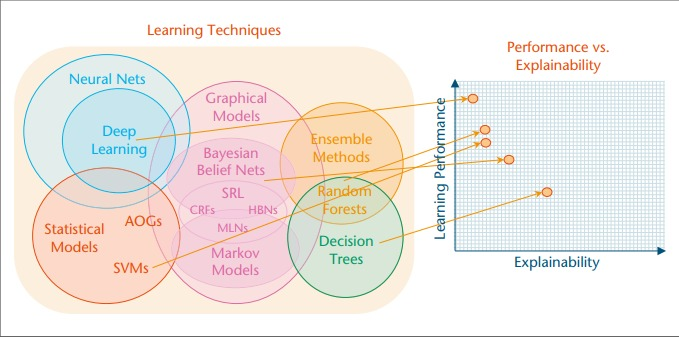
\includegraphics[width=0.72\textwidth]{figuras/Performance_Versus_Explainability.jpg}
    \caption[Relação entre performance e explicabilidade das técnicas de aprendizado de máquina]{Relação entre performance e explicabilidade das principais famílias de técnicas de aprendizado de máquina. À esquerda, as técnicas agrupadas por família; à direita, cada uma é posicionada em um plano cujo eixo horizontal é a explicabilidade e cujo eixo vertical é a performance do modelo (rotulada no original como \textit{learning performance}). Quanto mais alta e mais à esquerda a técnica, mais capaz de representar relações complexas e menos explicável ela é: redes de aprendizado profundo e métodos de \textit{ensemble}, como o XGBoost, ocupam o topo, enquanto árvores de decisão isoladas são mais explicáveis e menos precisas.}
    \label{fig:tradeoff}
    \small{Fonte: \cite{raizonvilleBlackBoxGlass2022}.}
\end{figure}


\section{O Custo Econômico e Estratégico da Interpretabilidade}
\label{sec:custo}

A decisão de restringir a tecnologia da administração tributária apenas a modelos simples e interpretáveis impõe um custo de oportunidade mensurável e significativo. Embora a transparência seja um requisito ético e legal, a literatura demonstra que a ``taxa de sacrifício'' em performance ao abandonar modelos de caixa-preta pode representar perdas milionárias em recuperação de crédito.

Raizonville e Lambin (2022) modelam a explicabilidade como uma decisão estratégica e demonstram quantitativamente que modelos de caixa-preta otimizados podem gerar um retorno sobre o investimento (ROI) superior na ordem de \textbf{15 a 20 pontos-base} em carteiras de crédito, comparado a modelos lineares tradicionais. Em escalas de dívida pública, essa diferença percentual traduz-se em montantes absolutos expressivos.

Um estudo empírico realizado por \citeonline{delangeExplainableAICredit2022} em um banco comercial norueguês quantificou o impacto financeiro dessa escolha tecnológica. Ao comparar um modelo de \textit{Light Gradient Boosting Machine} (similar ao XGBoost usado pela SEFAZ-DF) com uma Regressão Logística tradicional, os autores identificaram que o modelo avançado reduziu as perdas financeiras anuais entre \textbf{20 e 35 milhões de coroas norueguesas (aprox. 2 a 3,5 milhões de dólares)}. Essa economia decorreu tanto da redução de falsos negativos (inadimplentes não identificados) quanto da diminuição de falsos positivos (bons pagadores erroneamente classificados como risco).

Além do impacto direto na arrecadação, \citeonline{alonsoUnderstandingPerformance2021} indicam que o uso de técnicas avançadas de aprendizado de máquina pode levar a uma redução de \textbf{12,4\% a 17\% nos requisitos de capital regulatório} para instituições financeiras, devido à maior precisão na mensuração do risco. Esse achado também é retomado por \citeonline{schwartzEnhancingMLModels2025} no debate sobre performance e interpretabilidade.

No contexto da Dívida Ativa do Distrito Federal, esse ``custo da explicabilidade'' evidencia o risco de ineficiência alocativa. Utilizar modelos menos precisos apenas para satisfazer requisitos superficiais de transparência poderia aumentar a probabilidade de erros de classificação, como enquadrar contribuintes com potencial de recuperação em categorias de baixa recuperabilidade. Portanto, a literatura sugere que a solução economicamente viável não é reduzir a complexidade do modelo, mas sim investir em camadas computacionais que expliquem essa complexidade de forma \textit{pós-hoc} \cite{schmittExplainableAutomatedMachine2024}.


\section{Desbalanceamento de Dados e Avaliação da Performance do Modelo}
\label{sec:metricas}

A validação de modelos de pontuação de crédito (\textit{Credit Scoring}) e Dívida Ativa exige métricas que vão além da simples taxa de acerto, uma vez que as bases de dados tributárias são inerentemente desbalanceadas (a quantidade de bons pagadores difere drasticamente da de inadimplentes). Segundo \citeonline{changCreditRiskPrediction2024}, a escolha inadequada da métrica pode levar a uma falsa percepção de eficácia do modelo.

\subsection{Desbalanceamento Macro e Micro}
\label{subsec:desbalanceamento}

Uma base é desbalanceada quando os exemplos não estão distribuídos de forma equilibrada entre os grupos que o modelo precisa aprender. A literatura distingue dois níveis desse fenômeno \cite{heLearningImbalancedData2009}:

\begin{itemize}
    \item \textbf{Desbalanceamento macro (entre classes):} diferença de tamanho entre as classes da variável-alvo. No Rating, ele aparece em dois pontos. Na variável que o modelo aprende, a taxa histórica de pagamento das CDAs, registrada nos parâmetros do modelo de produção, é de apenas 15,2\% no ICMS, 19,7\% nas Taxas, 20,6\% no ISS, 26,3\% no IPVA e 36,6\% no IPTU; ou seja, para cada CDA paga há entre duas e seis não pagas. Na classificação final, as classes também são desiguais: na amostra sintética de ICMS analisada no Capítulo \ref{cap:resultados_analise}, a classe C reúne 62,9\% das CDAs, e a classe D, apenas 2,7\%.
    \item \textbf{Desbalanceamento micro (dentro das classes):} diferença de representação entre subgrupos de uma mesma classe. Mesmo que a classe ``pagou'' tenha muitos exemplos no total, eles podem estar concentrados em alguns perfis (por exemplo, empresas de grande porte ou imóveis de determinadas regiões administrativas) e ser raros em outros. Esses subgrupos pequenos, chamados na literatura de pequenos disjuntos (\textit{small disjuncts}), concentram uma parcela desproporcional dos erros de classificação \cite{joClassImbalancesSmall2004}. No Rating, o problema é agravado pelo \textit{target encoding}: categorias com poucas ocorrências, como um bairro com poucas CDAs, têm sua taxa de pagamento suavizada em direção à média geral, de modo que o modelo passa a tratar todos os contribuintes desse grupo como ``médios'', independentemente de seu comportamento real.
\end{itemize}

Os dois níveis produzem efeitos diferentes. O desbalanceamento macro faz o modelo favorecer a classe majoritária: como errar a classe rara pesa pouco no erro total do treinamento, o modelo pode aprender a quase nunca prevê-la. O desbalanceamento micro é mais difícil de perceber, porque o modelo pode ter boa performance média e, ao mesmo tempo, errar sistematicamente para um subgrupo pequeno. Quando esse subgrupo coincide com um recorte social (região, porte, tipo de contribuinte), o erro passa a ser também um problema de justiça, tratado na Seção \ref{subsec:vies_metricas}. O efeito do desbalanceamento micro sobre um modelo treinado com os dados deste trabalho é medido experimentalmente na Seção \ref{sec:resultado_desbalanceamento}.

\subsection{Matriz de Confusão e Métricas Derivadas}
A base para a avaliação de classificadores binários é a Matriz de Confusão, que cruza as predições do modelo com a realidade fiscal, gerando quatro resultados possíveis: Verdadeiros Positivos ($VP$), Verdadeiros Negativos ($VN$), Falsos Positivos ($FP$) e Falsos Negativos ($FN$).

\begin{itemize}
    \item \textbf{Acurácia (\textit{Accuracy}):} Mede a proporção global de acertos.
    \begin{equation}
        ACC = \frac{VP + VN}{VP + VN + FP + FN}
    \end{equation}
    \textbf{Limitação:} Em bases desbalanceadas, a acurácia é enganosa. Se 95\% dos contribuintes são inadimplentes, um modelo ``ingênuo'' que classifique \textit{todos} como inadimplentes terá 95\% de acurácia, mas será inútil para identificar os 5\% de bons pagadores (o ``Paradoxo da Acurácia'') \cite{noriegaMachineLearningCredit2023}.

    \item \textbf{Revocação ou Sensibilidade (\textit{Recall}):} Mede a capacidade do modelo de detectar a classe de interesse (ex: identificar corretamente quem vai pagar a dívida).
    \begin{equation}
        Recall = \frac{VP}{VP + FN}
    \end{equation}
    \textbf{Importância:} No contexto da SEFAZ, um baixo \textit{Recall} significa perder a oportunidade de cobrar um contribuinte que teria capacidade de pagamento (Falso Negativo), gerando perda direta de receita.

    \item \textbf{Precisão (\textit{Precision}):} Mede, entre os casos classificados como positivos pelo modelo, quantos de fato pertencem à classe positiva.
    \begin{equation}
        Precision = \frac{VP}{VP + FP}
    \end{equation}
    \textbf{Importância:} No contexto da SEFAZ, baixa precisão significa direcionar esforços de cobrança a contribuintes com menor probabilidade de recuperação, consumindo recursos administrativos sem retorno proporcional.

    \item \textbf{F1-Score:} É a média harmônica entre a Precisão (qualidade do acerto) e o \textit{Recall} (quantidade de acertos).
    \begin{equation}
        F1 = 2 \cdot \frac{Precision \cdot Recall}{Precision + Recall}
    \end{equation}
    Esta métrica é preferível em cenários fiscais, pois penaliza modelos muito imprecisos ou que omitem muitos devedores (baixo recall).
\end{itemize}

\subsection{Médias Micro e Macro das Métricas}

Quando há mais de duas classes, como as quatro classes do Rating, as métricas acima são calculadas para cada classe $k$ e precisam ser resumidas em um único número. Há duas formas de fazê-lo, e a diferença entre elas é justamente o que revela o efeito do desbalanceamento \cite{sokolovaSystematicAnalysisPerformance2009}:

\begin{itemize}
    \item \textbf{Média micro:} soma os acertos e erros de todas as classes antes de calcular a métrica. Cada CDA tem o mesmo peso, de modo que o resultado é dominado pelas classes mais numerosas:
    \begin{equation}
        Precision_{micro} = \frac{\sum_{k} VP_k}{\sum_{k} (VP_k + FP_k)}
    \end{equation}
    \item \textbf{Média macro:} calcula a métrica separadamente em cada uma das $K$ classes e tira a média simples. Cada classe tem o mesmo peso, independentemente do tamanho:
    \begin{equation}
        F1_{macro} = \frac{1}{K} \sum_{k=1}^{K} F1_k
    \end{equation}
\end{itemize}

Um modelo que acerta bem as classes grandes e falha nas pequenas apresenta média micro alta e média macro baixa. No exemplo do ICMS, um classificador que atribuísse C a todas as CDAs teria média micro próxima de 63\% e $F1$ igual a zero nas classes A, B e D, o que derrubaria a média macro. A mesma lógica pode ser aplicada a subgrupos de contribuintes, em vez de classes: calcular a métrica separadamente por região, por porte ou por imposto expõe o desbalanceamento micro que a média geral esconde.

\subsection{Curva ROC e Área sob a Curva (AUC-ROC)}
A Área sob a Curva ROC (AUC-ROC) mede a capacidade do modelo de distinguir entre classes ao longo de diferentes limiares de decisão. A curva ROC relaciona a taxa de verdadeiros positivos à taxa de falsos positivos, resumindo o comportamento do classificador em múltiplos pontos de corte \cite{noriegaMachineLearningCredit2023, changCreditRiskPrediction2024}.

\begin{equation}
    TPR = \frac{VP}{VP + FN}
\end{equation}

\begin{equation}
    FPR = \frac{FP}{FP + VN}
\end{equation}

Quanto mais a curva se aproxima do canto superior esquerdo do gráfico ROC, melhor é a capacidade discriminatória do modelo. Em termos sintéticos, quanto mais próxima de 1 for a AUC-ROC, maior é a probabilidade de o classificador atribuir maior risco aos casos efetivamente problemáticos do que aos casos regulares.


\section{Inteligência Artificial Explicável como Solução de Governança}
\label{sec:xai}

Para resolver o conflito entre a performance do modelo e a transparência, a literatura propõe o uso de métodos de Inteligência Artificial Explicável (XAI, do inglês \textit{Explainable Artificial Intelligence}). \citeonline{maratheDemystifyingInterpretableAI} realiza uma revisão crítica dessas técnicas no setor financeiro, destacando duas abordagens principais: LIME e SHAP. A escolha entre elas é crítica para a segurança jurídica e a auditabilidade das decisões fiscais. Esta seção apresenta não apenas os fundamentos conceituais dessas metodologias, mas também seu detalhamento algorítmico, essencial para a compreensão de sua aplicação prática na administração tributária.

\subsection{O Problema da Caixa-Preta e a Proposta da Inteligência Artificial Explicável}

O problema central que a Inteligência Artificial Explicável busca resolver é a \textit{opacidade cognitiva}. Modelos avançados, como redes neurais e \textit{Gradient Boosting}, realizam milhões de operações matemáticas internas para chegar a um resultado. Para um ser humano, esse processo é inescrutável — uma verdadeira ``caixa-preta'' onde a lógica de decisão é inacessível \cite{molnarInterpretableMachineLearning}.

A proposta da Inteligência Artificial Explicável é atuar como uma ``ponte'' ou uma interface tradutora. Segundo \citeonline{reddyBridgingAIHuman2024}, o objetivo dessa abordagem não é simplificar o modelo matemático em si, o que reduziria sua precisão, mas fornecer uma camada interpretativa capaz de traduzir as correlações complexas do algoritmo em justificativas causais inteligíveis para humanos (ex: ``O risco foi considerado alto \textit{porque} o valor da dívida excede a média do setor'').

No contexto da administração pública, a Inteligência Artificial Explicável deixa de ser apenas uma ferramenta de depuração de código para se tornar um instrumento de governança algorítmica. Ela permite que o Estado mantenha a eficiência da IA enquanto restaura a \textit{accountability} (responsabilização) e o direito ao contraditório, transformando a ``caixa-preta'' em uma ``caixa de vidro'' auditável \cite{raizonvilleBlackBoxGlass2022}.

\subsection{LIME: Aproximação Linear Local por Perturbação}
\label{subsec:lime}

O método LIME (\textit{Local Interpretable Model-agnostic Explanations}), introduzido no trabalho seminal de \citeonline{ribeiroWhyShouldTrust2016}, propõe uma abordagem agnóstica ao modelo para explicar predições individuais. A premissa fundamental é que, embora a fronteira de decisão de um modelo complexo $f(x)$ (como o XGBoost) seja altamente não-linear e complexa globalmente, ela pode ser aproximada por uma função linear simples $g(x)$ em uma vizinhança local infinitesimal ao redor de uma instância de interesse. 

Apesar de ser eficiente para análises exploratórias rápidas, \citeonline{maratheDemystifyingInterpretableAI} e \citeonline{reddyBridgingAIHuman2024} alertam para a \textbf{instabilidade inerente ao LIME}: pequenas variações na definição da ``vizinhança'' ou na amostragem de dados podem gerar explicações contraditórias para instâncias similares. No contexto de uma auditoria fiscal, essa falta de consistência pode fragilizar a defesa administrativa do \textit{rating}.

\subsubsection{Detalhamento Algorítmico do LIME}

O fluxo de execução do algoritmo para explicar a classificação de um contribuinte específico ocorre em cinco etapas distintas, conforme ilustrado conceitualmente na Figura \ref{fig:lime_fluxo}:

\begin{enumerate}
    \item \textbf{Seleção da Instância ($x$):} Seleciona-se o vetor de variáveis explicativas do contribuinte cujo \textit{rating} se deseja explicar.
    
    \item \textbf{Amostragem por Perturbação:} O algoritmo gera um novo conjunto de dados sintéticos $Z$.  Para dados tabulares, isso é realizado perturbando os atributos de $x$ (adicionando ruído gaussiano a variáveis contínuas ou alterando categorias), criando permutações $z'$ próximas ao original. 
    
    \item \textbf{Predição pelo Modelo Caixa-Preta:} O modelo original complexo $f$ é utilizado como um ``oráculo'' para prever o resultado dessas instâncias sintéticas, gerando um vetor de predições $f(z')$.
    
    \item \textbf{Ponderação por Proximidade ($\pi_x$):} Calcula-se a distância euclidiana ou de cosseno entre a instância original $x$ e cada instância gerada $z'$. Atribui-se um peso $\pi_x(z)$ maior para as instâncias mais próximas e menor para as distantes, geralmente utilizando um kernel exponencial:
    \begin{equation}
        \pi_x(z) = \exp\left(-\frac{D(x, z)^2}{\sigma^2}\right)
    \end{equation}
    Onde $D$ é a função de distância e $\sigma$ é a largura do kernel.
    
    \item \textbf{Treinamento do Modelo Explicador (Surrogate):} Treina-se um modelo interpretável $g$ (geralmente uma regressão linear ponderada ou Lasso) que tenta minimizar o erro em relação às predições de $f$ dentro da vizinhança ponderada. 
\end{enumerate}

O objetivo matemático do LIME é encontrar o modelo $g$ que minimiza a seguinte função objetivo:

\begin{equation}
    \xi(x) = \operatorname*{argmin}_{g \in G} \ \mathcal{L}(f, g, \pi_x) + \Omega(g)
\end{equation}

Onde:
\begin{itemize}
    \item $\mathcal{L}$ é a função de perda (como o erro quadrático médio) que mede a infidelidade de $g$ em relação a $f$, ponderada pela proximidade $\pi_x$.
    \item $\Omega(g)$ é uma medida de complexidade do modelo explicador (ex: número de coeficientes não nulos na regressão), garantindo que a explicação gerada seja, de fato, inteligível para o auditor fiscal.
\end{itemize}

\begin{figure}[H]
  \centering
  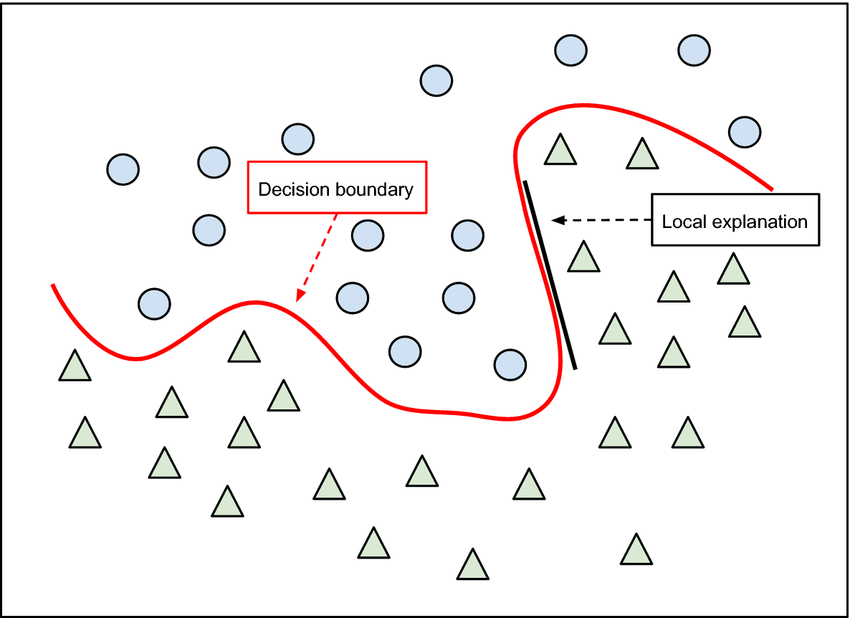
\includegraphics[width=0.6\textwidth]{figuras/lime.png}
  \caption[Intuição do LIME: ajuste linear local em uma fronteira de decisão complexa]{Intuição do LIME. Círculos e triângulos representam exemplos de duas classes, e a curva vermelha é a fronteira de decisão de um modelo complexo, que não pode ser descrita por uma regra simples. O LIME não tenta explicar a fronteira inteira: ele aproxima apenas o trecho próximo à instância de interesse por uma reta (segmento preto, ``explicação local''), cujos coeficientes indicam quais variáveis empurram aquela instância para cada lado. A explicação vale somente nessa vizinhança.}
  \label{fig:lime_fluxo}
  \small{Fonte: \citeonline{ribeiroWhyShouldTrust2016}.}
\end{figure}

\subsection{SHAP: Consistência via Teoria dos Jogos}
\label{subsec:shap}

Para superar a instabilidade estocástica do LIME, \citeonline{lundbergUnifiedApproachInterpreting2017} propuseram o SHAP (\textit{SHapley Additive exPlanations}). Este método unifica a interpretabilidade em aprendizado de máquina com a Teoria dos Jogos Cooperativos, desenvolvida pelo Nobel de Economia Lloyd Shapley em 1953. Conceitualmente, o SHAP calcula a contribuição marginal média de cada variável para a nota final do \textit{rating}, considerando todas as combinações possíveis de fatores \cite{nallakaruppanCreditRiskAssessment2024}.

No contexto da classificação de dívida ativa, a predição do modelo é tratada como um ``jogo'' cujo objetivo é gerar a pontuação de risco. As ``jogadoras'' são as variáveis explicativas do contribuinte, como valor da dívida e tempo de atraso. O Valor de Shapley calcula a contribuição marginal média de cada variável para o resultado final, considerando todas as combinações possíveis de variáveis.

\subsubsection{Detalhamento Algorítmico e Fórmula Matemática}

O cálculo exato do valor SHAP ($\phi_i$) para uma variável $i$ é dado pela média ponderada das contribuições marginais dessa variável em todos os subconjuntos possíveis $S$ do conjunto total de variáveis $F$:

\begin{equation}
    \phi_i(f, x) = \sum_{S \subseteq F \setminus \{i\}} \frac{|S|! (|F| - |S| - 1)!}{|F|}! [f_x(S \cup \{i\}) - f_x(S)]
\end{equation}

Onde:
\begin{itemize}
    \item $S \subseteq F \setminus \{i\}$ indica que $S$ representa qualquer subconjunto de variáveis que não contém a variável $i$.
    \item $|S|$ representa a quantidade de elementos do subconjunto $S$, enquanto $|F|$ representa o número total de variáveis do modelo.
    \item O símbolo $\sum$ indica a soma das contribuições marginais calculadas para todos os subconjuntos possíveis.
    \item $f_x(S)$ é a predição do modelo utilizando apenas as variáveis presentes no subconjunto $S$. Como o modelo original geralmente requer todas as variáveis, as variáveis ausentes são marginalizadas, isto é, substituídas por valores médios ou amostras de fundo.
    \item $f_x(S \cup \{i\}) - f_x(S)$ representa a contribuição marginal, isto é, o quanto a predição muda quando a variável $i$ é adicionada ao grupo $S$.
\end{itemize}

\subsubsection{TreeSHAP e Otimização Computacional}

Devido ao custo computacional exponencial ($2^F$) da fórmula exata, inviável para modelos com muitas variáveis, utiliza-se neste trabalho a variante \textbf{TreeSHAP}, específica para modelos baseados em árvores (\textit{Gradient Boosting}). O TreeSHAP explora a estrutura hierárquica das árvores de decisão para calcular os valores exatos de Shapley em tempo polinomial $O(TLD^2)$, onde $T$ é o número de árvores, $L$ o número máximo de folhas e $D$ a profundidade máxima \cite{lundbergUnifiedApproachInterpreting2017}. 

\subsubsection{Visualização e Propriedades Axiomáticas}

A lógica de funcionamento do SHAP pode ser visualizada na \textbf{Figura \ref{fig:shap_waterfall}}, que apresenta um gráfico de cascata (\textit{waterfall plot}). Neste exemplo, a predição inicia-se na média global do modelo (valor esperado $E[f(x)]$). Em seguida, cada barra horizontal representa a contribuição marginal da variável, elevando ou reduzindo a pontuação final da predição. O valor final $f(x)$ é, portanto, a soma matemática exata dessas contribuições individuais.

\begin{figure}[H]
    \centering
    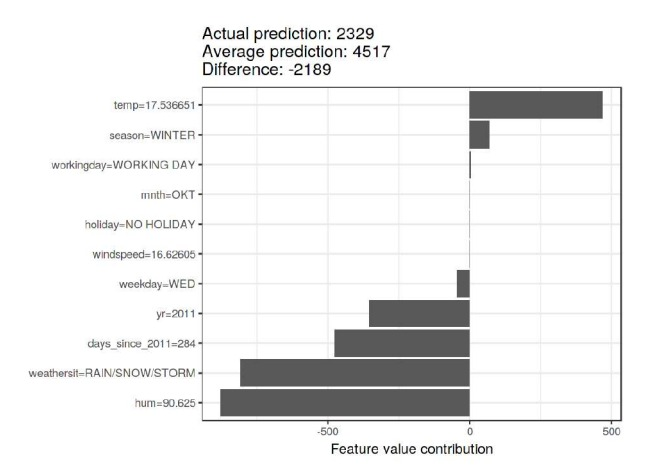
\includegraphics[width=0.9\textwidth]{figuras/watterfall_plot.jpg}
    \caption[Decomposição de uma predição individual com valores de Shapley]{Decomposição de uma predição individual com valores de Shapley, em um exemplo de previsão do número de bicicletas alugadas em um dia. O topo informa a predição do modelo para esse dia (2.329), a predição média (4.517) e a diferença entre elas ($-2.189$). Cada barra é a contribuição de uma variável, com seu valor observado à esquerda: barras para a direita aumentam a predição, e barras para a esquerda a reduzem. A soma de todas as barras é exatamente a diferença informada no topo; neste caso, a umidade alta e o tempo chuvoso explicam a maior parte da queda.}
    \label{fig:shap_waterfall}
    \small{Fonte: \citeonline{molnarInterpretableMachineLearning}.}
\end{figure}

\citeonline{shreyaExplainableArtificialIntelligence2025} enfatizam que essa propriedade de aditividade, demonstrada visualmente acima, é o que garante a consistência da explicação e satisfaz axiomas essenciais:
\begin{enumerate}
    \item \textbf{Eficiência:} A soma das barras (contribuições) explica exatamente o desvio da predição em relação à média. 
    \item \textbf{Consistência:} Se o modelo altera o peso de uma variável, o tamanho da barra no gráfico reflete essa mudança proporcionalmente.
    \item \textbf{Simetria:} Variáveis que contribuem igualmente recebem valores SHAP iguais.
    \item \textbf{Dummy (Nulidade):} Variáveis que não influenciam a predição recebem valor SHAP igual a zero.
\end{enumerate}

Essas propriedades indicam que o SHAP é uma ferramenta adequada e tecnicamente consistente para justificar administrativamente a classificação de risco da SEFAZ-DF, permitindo ao auditor fiscal decompor a nota do \textit{rating} em parcelas exatas atribuíveis a cada fator \cite{molnarInterpretableMachineLearning}.

\subsection{Análise Comparativa e Justificativa da Escolha}
\label{subsec:comparacao_xai}

A Tabela \ref{tab:shap_vs_lime} consolida as diferenças fundamentais entre as duas abordagens, destacando as vantagens do SHAP em termos de consistência para fins de auditoria e segurança jurídica.

\begin{table}[H]
    \centering
    \caption[Comparação técnica entre LIME e SHAP]{Comparação técnica entre LIME e SHAP segundo oito critérios relevantes para a auditoria fiscal. Cada linha contrapõe as duas técnicas em um critério: fundamento teórico, garantias formais, consistência, custo computacional, reprodutibilidade, forma de interpretação, segurança jurídica e papel sugerido no contexto da SEFAZ-DF. Em síntese, o LIME é mais simples e rápido, porém estocástico; o SHAP é determinístico e tem garantias axiomáticas, sendo mais adequado à justificativa formal de um \textit{rating}.}
    \label{tab:shap_vs_lime}
    \small
    \renewcommand{\arraystretch}{1.3} % Aumenta o espaçamento entre linhas para melhor leitura
    \begin{tabular}{p{3.5cm} p{5.0cm} p{5.0cm}}
        \toprule
        \textbf{Critério} & \textbf{LIME} & \textbf{SHAP} \\
        \midrule
        \textbf{Fundamentação} & Aproximação linear local via perturbação & Teoria dos Jogos Cooperativos (Valores de Shapley) \\
        \textbf{Garantias Axiomáticas} & Nenhuma garantia formal & Eficiência, Simetria, Dummy e Aditividade \\
        \textbf{Consistência} & Baixa (sensível a amostragem e parâmetros do kernel) & Alta (única solução que satisfaz os axiomas de justiça) \\
        \textbf{Complexidade} & Baixa a Média ($O(N \cdot M)$) & Alta (exata) / Otimizada ($O(TLD^2)$ via TreeSHAP) \\
        \textbf{Reprodutibilidade} & Estocástica (pode variar entre execuções) & Determinística (mesmo resultado sempre) \\
        \textbf{Interpretação} & Pesos de um modelo linear local & Contribuição marginal para o desvio da média \\
        \textbf{Segurança Jurídica} & Questionável (instabilidade) & Robusta (consistência matemática auditável) \\
        \textbf{Uso na SEFAZ-DF} & Diagnóstico exploratório rápido & Justificativa formal de \textit{ratings} \\
        \bottomrule
    \end{tabular}
    \vspace{0.2cm}
    \footnotesize{\\ \textbf{Fonte:} Elaborado pelos autores com base em \citeonline{molnarInterpretableMachineLearning} e \citeonline{lundbergUnifiedApproachInterpreting2017}.}
\end{table}

A análise comparativa evidencia que, para o contexto específico da SEFAZ-DF, o \textbf{SHAP apresenta vantagens relevantes}. A consistência determinística e as garantias axiomáticas são requisitos fundamentais quando as explicações geradas pelo modelo podem ser objeto de contestação administrativa ou judicial. Um contribuinte que questione seu \textit{rating} tem direito a uma explicação reproduzível e matematicamente fundamentada, e o SHAP oferece atributos compatíveis com essa exigência.

Isso não invalida o uso do LIME como ferramenta complementar para análises exploratórias iniciais ou para comunicação simplificada com partes interessadas não técnicas. Contudo, para a documentação oficial e a motivação formal dos atos administrativos de classificação de risco, o SHAP tende a ser a metodologia de referência.